\begin{frame}{2D OTFP: Transport Minimum Free-Energy Pathways}
\begin{tikzpicture}
\pcuad{\textwidth}{\textheight}
%\showcuad
\path(nw) +(0,0.2) node(cite)[anchor=north west]{\tiny \textcolor{red!80!black}{S. A. Paz, L. Maragliano, and CFA {\em J. Chem. Theory. Comput.} {\bf 14}:2743-2750 (2018)}};
\path(nw) +(0,0) node(image)[anchor=north west]{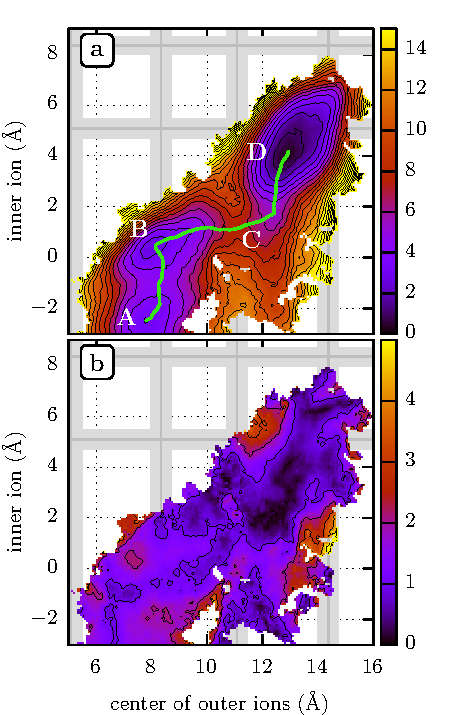
\includegraphics[width=0.5\textwidth]{fullfes_path_err.pdf}};
\path(nw) +(1.5,-4) node(errlab)[anchor=north west]{Error, $N$=3};
\path(nw) +(5,-1.5) node(bullets)[anchor=north west,text width=0.5\textwidth]{\begin{itemize}
\item A$\rightarrow$B: Innermost ion moves up one position
\item B$\rightarrow$C: CM$_{2,3}$ moves up one position, followed quickly by
\item C$\rightarrow$D: Innermost ion moves up one more position
\item $\Rightarrow$ Net translocation of one K$^+$
\item What role is water playing?
\end{itemize}};
\end{tikzpicture}
\end{frame}

